\documentclass[../main.tex]{subfiles}
\usepackage{silence}
\WarningFilter{glossaries}{No \printglossary or \printglossaries found}

\begin{document}
\ifSubfilesClassLoaded{%
    \graphicspath{{figures/6-CrossAttOmicsGate/}}%
    \setcounter{chapter}{5}%
}{
    \graphicspath{{../figures/6-CrossAttOmicsGate/}}%
}
\chapter{CrossAttOmicsGate}\label{chap:crossattomicsgate}
\minitocpage

\section{Method}
 Initially, an encoder independently projects each modality into a representational space, utilizing a self-attention mechanism to capture intra-modality interactions.
 Subsequently, the architecture employs cross-attention modules to represent modality pairs, focusing on inter-modality interactions.
 As the dimensionality of omics data is high, computing attention matrices directly is not feasible.
 We used a data decomposition strategy into groups to address this challenge, effectively reducing the memory demands associated with attention calculations~\cite{AttOmics}.

 \begin{figure}[htbp]
     \centering
     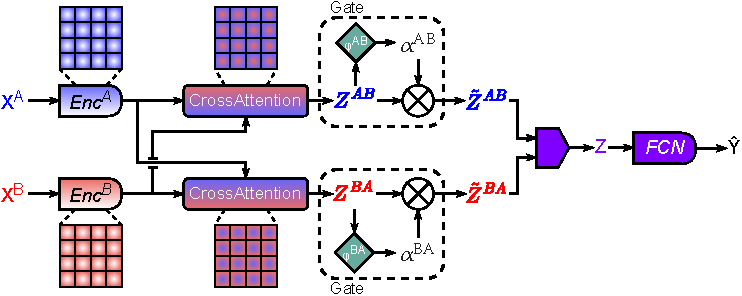
\includegraphics[width=\textwidth]{CrossAttOmicsGate.pdf}
     \caption{Model Architecture. Each modality \(X^i\) is encoded with an attention-based encoder. Modalities interactions are computed with cross-attention. A gating mechanism is used to select the most important interactions. The multimodal embedding is then obtained by concatenating the gated cross-attention outputs. A linear projection is then used to obtain predictions.}
     \label{fig:arch}
 \end{figure}

 \subsection{Modality encoders}
     In this section, we describe attention-based modality encoders that encode individual modalities.

     Let \( X = \left\{X^{1}, \cdots, X^{M} \right\} \) be a multimodal training example, where \(M\) is the number of modalities and \(Y\) is the associated label.
     We denote with \(X^{i} \in \symbb{R}^{p_i}\) each modality input, and $p_i$ is the number of features for modality $i$.
     Each modality input \(X^{i}\) is encoded with a self-attention-based encoder: \(\enc^{i}\)~\cite{AttOmics}.

     The omics profile \(X^{i} \in \symbb{R}^{p_i} \) is reshaped to a set of $k^i$ groups of similar sizes~(\cref{eq:attomics_groups}).
     \begin{equation}
         X^{i}_{G} = \left\{X^{i}_{g_j} \right\}_{1\leq j\leq k^i}\label{eq:attomics_groups}
     \end{equation}
     Each group vector $X^{i}_{g_j}$ is projected into an $s^i$-dimensional space with a trainable projection \(\phi^i\) (\cref{eq:attomics_groups_proj}).
     \begin{equation}
         X^{'i}_{G} = \left\{\phi^i\left(X^{i}_{g_j} \right) \right\}_{1\leq j\leq k^i}\label{eq:attomics_groups_proj}
     \end{equation}
     \Gls{mhsa} is then applied to each group \(g^i_j\)~(\(1 \leq j \leq k^i \)) to compute a new representation \({U^i = \left\{ U^i_{g_j}\right\}_{1 \leq j \leq k^i}}\) considering interactions between groups of the i-th modality.
     In each attention head,
     \begin{equation}
         U^{i}_{g_j} = A^{i}_{g_j} \cdot \left[ X_{g_1}' \cdot W^V, \cdots ,  X_{g_{k^i}}' \cdot W^V\right]^T \text{,}\label{eq:enc_mhsa}
     \end{equation}
     where $A^{i}_{g_j}$ is the attention vector computed by the usual dot product attention~\cite{AttentionAllYouNeed}.

     Each modality $i$ is represented in a lower dimensional space: \(U^{i} = \enc^{i}\left(X^{i}\right)\).
     Combining the different representations makes it possible to exploit their complementarity and redundancy.

 \subsection{CrossAttention: modalities interactions}
     The CrossAttention module is used to encode the interaction of two modalities.

     Cross-attention is applied to construct a new representation in which a target modality is reinforced by features from a source modality.
     The cross-attention is applied to all pairs of modalities, representing \(n_{\alpha}\) interactions to consider.
     Let us consider two modalities, a source \(i\) and a target \(j\), \(i \neq j\), which are encoded with their respective encoders to obtain the new representations \(U^i\) and \(U^j\).
     Cross-attention is performed with $H$ heads that learn different types of cross-modal interactions.
     For each head, cross-attention is applied to each group of the modalities \(g_p\) in order to obtain:
     \[ Z^{i\rightarrow j} = \left\{ Z^{i\rightarrow j}_{g_p} \in \symbb{R}^{l^j} \right\}_{1 \leq p \leq k^j}\text{,}\]
     where $l^j = \frac{s^j}{H} \in \symbb{N}$.
     \( Z^{i\rightarrow j}\) has the same number of groups as the target modality $j$.

     \(Z^{i\rightarrow j}_{g_p}\) is obtained by applying the scale dot product attention~\cite{AttentionAllYouNeed} where the source modality \(i\) is used as the key and value.
     The target modality \(j\) is used as the query.
     The vectors \(Z^{i\rightarrow j}_{g_p}\) are concatenated into a new vector \(Z^{ij}\).

 \subsection{Gating}
     The gating mechanism is used to select the most important interactions.

     The multimodal embedding \(Z^{ij}\) is projected to a single neuron by a trainable projection \(\phi_{\alpha^{ij}}\) followed by a sigmoid activation \(\sigma\) to obtain the gating parameters \(\alpha^{ij} = \left[\alpha^{ij}_{k}\right]\), \(1 \leq k \leq n_b\) where \(n_b\) is the size of a batch:
     \begin{equation}
         \alpha^{ij} = \sigma \left( \phi_{\alpha^{ij}}\left( Z^{ij} \right)\right)
         \label{eq:gate_alpha}
     \end{equation}
     Each \(\alpha^{ij}_{k}\) represents the importance of the considered modality interactions for a sample \(k\) in the current batch.
     For each sample \(k\), there are \(n_{\alpha}\) interactions to consider.
     The projection \(\phi_{\alpha^{ij}}\) is initialized in such a way that each interaction has the same importance scores at the beginning of the training, i.e., a value of 0.5.
     Then, the importance score is combined with the cross-attention output in a multiplicative manner:
     \[ \tilde{Z}^{ij} = \alpha^{ij} \odot Z^{ij} \]

 \subsection{Predictor module}

     All \(\tilde{Z}^{ij}\) embeddings are concatenated to form a single multimodal vector $Z$.
     The vector $Z$ is then fed to a \gls{fcn} to obtain the prediction $\hat{Y}$.

     The output layer has one neuron per class, and a $\operatorname{softmax}$ activation function is applied to get the probability vector ${P = \left[p_c\right]_{1\leq c\leq C}}$, where $C$ denotes the number of classes.

 \subsection{Model training}
     We adopt a two-phase training procedure.
     In the first step, each modality encoder $\enc^i$ is trained individually to learn a compact representation of the modality $i$ by adding an \gls{fcn} layer with one neuron per class and a $\operatorname{softmax}$ activation function.
     Each encoder is trained end-to-end with a weighted cross-entropy loss to account for class imbalance:
     \begin{equation*}
         \symcal{L}_{CE}(\theta^{i}) = - \sum_{c=1}^{C}w_c Y_c \log\left( \fcn\left(\enc^{i}\left(X^{i}, \theta^{i}\right)\right)\right) \text{,}
     \end{equation*}
     where \( \theta^{i}\), are the parameters associated with the encoder \(\enc^{i}\) and \(w_c\) denotes the weight\footnote{inversely proportional to the class size} of class $c \in \left\{1, \cdots,C \right\}$.

     In a second step, we freeze the encoder parameters \(\theta^i\), and train the multimodal weights of the model, i.e. all the cross-attention and the predictor module weights.
     The training on the predictive task is done with a weighted cross-entropy loss:
     \begin{equation*}
         \symcal{L}_{CE}(\theta) = - \sum_{c=1}^{C}w_c Y_c \log\left( p_c\right) \text{,}
     \end{equation*}
     where $\theta$ denotes the multimodal parameters, i.e., the cross-attention and predictor parameters.
     To have an interpretable model, the \(\alpha^{ij}\) values must be sparse.
     We want to select only the relevant interactions for each sample.
     In addition, the selected \(\alpha^{ij}\) must be diverse across samples; samples should have different important interactions.
     In order to favor sparse and diverse values of the importance scores \(\alpha^{ij}\), we added four penalty terms: \(\symcal{L}_{01}\) and \(\symcal{L}_{b}\) that ensure sparsity, \(\symcal{L}_{e}\) and \(\symcal{L}_{v}\) that force the diversity.
     \(\symcal{L}_{b}\) and \(\symcal{L}_{e}\) depends on a sparsity term \(\tau\).

     The \(\symcal{L}_{01}\) is based on the loss used in FairDARTS~\cite{FairDARTS} to push the sigmoid value of \(\alpha^{ij}\) towards 0 or 1 in order to eliminate the ambiguities regarding the significance of the interactions between modalities \(i\) and \(j\):
     \[ \symcal{L}_{01} = - \frac{1}{n_{b}}\sum_{k}^{n_b}\frac{1}{n_{\alpha}}\sum_{\substack{i,j \\ i \neq j}} \left( \alpha_k^{ij} - 0.5 \right)^2 \]

     Combined with the term \(\symcal{L}_{01}\), the term \(\symcal{L}_{e}\), constrains the \(\alpha^{ij}\) values to have the desired sparsity \(\tau\)~\cite{Bengio2015ConditionalCI}.

     \[ \symcal{L}_{e} = \frac{1}{n_b} \sum_{k}^{n_b} \left\| \left(\frac{1}{n_{\alpha}}\sum_{\substack{i,j \\ i \neq j}} \alpha^{ij}_{k}\right) - \tau \right\|_2\]

     Using only the terms \(\symcal{L}_{01}\) and \(\symcal{L}_{e}\), a valid solution would be to select some of the \(\alpha^{ij}\) with a high probability and ignore the others for any samples.
     Indeed, all \(\alpha^{ij}\) can not be equally selected during the training, limiting the diversity of selected interactions across patients.
     To avoid this problem, the terms \(\symcal{L}_{b}\) and \(\symcal{L}_{v}\) are used.
     The term \(\symcal{L}_{b}\) ensures that each \(\alpha^{ij}\) can be used with a probability \(\tau\)~\cite{Bengio2015ConditionalCI}.

     \[ \symcal{L}_{b} = \sum_{\substack{i,j \\ i \neq j}} \left\|\frac{1}{n_b}\sum_{k}^{n_b}\alpha^{ij}_k - \tau \right\|_2\]

     The term \(\symcal{L}_{v}\) aims to maximize the variances of \(\alpha^{ij}\) across the data.
     This term ensures that the model is not learning a uniform distribution of \(\alpha^{ij}\) across samples.
     \[ \symcal{L}_{v} = - \sum_{\substack{i,j \\ i \neq j}} \operatorname{var}_k\left\{\alpha^{ij}_{k} \right\}\]
     The diversity constraints, represented by the terms \(\symcal{L}_{b}\) and \(\symcal{L}_{v}\) forces the network to learn a set of sample-specific interactions.

     In the second step, the total loss, \(\symcal{L}_{total}\), that the network is trained on, is the sum of the task loss \(\symcal{L}_{CE}\) and the different regularization terms:
     \[ \symcal{L}_{total} = \symcal{L}_{CE}\left(\theta\right) + w_{01}\symcal{L}_{01} + w_{v}\symcal{L}_{v} + w_{e}\symcal{L}_{e} + w_{b}\symcal{L}_{b}\]


\section{Results}
 \subsection{Dataset}
     Despite the development of high-throughput methods, there are few large multiomics datasets.
     Such datasets are difficult to obtain as they require patient approbation and standardized procedure across multiple sites with extensive computing resources to process the large amount of data produced.
     \Gls{tcga}~\cite{TCGA} dataset is the largest one available to date.
     We collected DNA methylation (DNAm), gene expression (mRNA), miRNA expression data, copy number variation (CNV), and proteomics for 5862 patients of 18 different cancers from the GDC Data Portal\footnote{\url{https://portal.gdc.cancer.gov/}}.
     We considered the \(\beta\)-value average of all probes located within 1500 base pairs of gene transcription start site as the methylation features.
     No feature selection was applied, and data were standardized to a zero mean and unit variance.
     We considered coding and non-coding mRNA (nc mRNA) as two different modalities, as nc mRNAs can affect cancer cell fate through various mechanisms~\cite{Grillone2020}.

     70\% of the data was used as a training set, 15\% forms the validation set, and the remaining 15\% forms the test set while preserving the proportion of each cancer.
     This dataset is used on a classification task, predicting each patient's cancer type.
     The task was evaluated with the accuracy metric.

 \subsection{Gating mechanism improves accuracy}
     \begin{figure}[htbp]
         \centering
         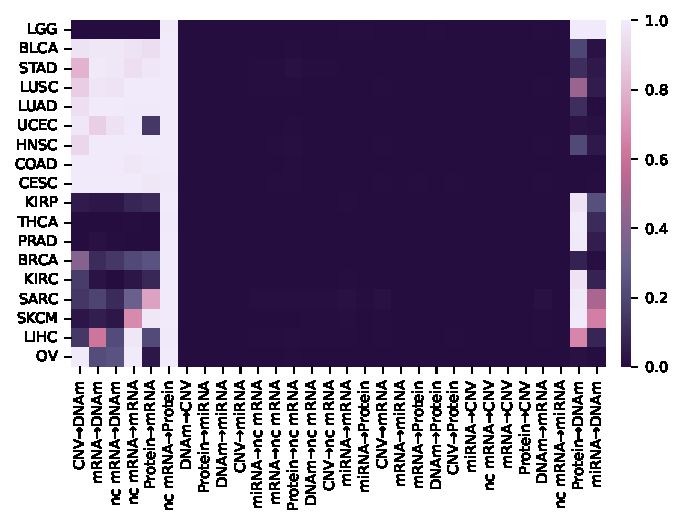
\includegraphics[scale=0.83]{signature_alphas.pdf}
         \caption{Visualization of how the different \(\alpha^{ij}\) are used among the different classes.}
         \label{fig:alphas_signature}
     \end{figure}

     We choose the same model architecture without the gating mechanism as a baseline.
     Adding the gating mechanism does not significantly change the number of parameters, ensuring a fair comparison.

     We first evaluated the impact of the gating on the accuracy when predicting the type of cancer.
     \Cref{tab:base_table} shows the accuracy obtained with the baseline model (no gate) and the gated model (gate).
     The model with the gating mechanism slightly outperforms the baseline approach.

     \begin{table}[htbp]
        \sisetup{separate-uncertainty-units=single, separate-uncertainty,detect-mode}
         \centering
         \caption{Impact of the gating mechanism on the accuracy}\label{tab:base_table}
         \begin{tblr}{
            colspec={
                Q[l,m]
                Q[si={table-format=1.3(3),table-number-alignment=center, table-align-uncertainty = true}]
                Q[si={table-format=1.3(3),table-number-alignment=center, table-align-uncertainty = true}]
                Q[si={table-format=1.3(3),table-number-alignment=center, table-align-uncertainty = true}]
                Q[si={table-format=1.3(3),table-number-alignment=center, table-align-uncertainty = true}]
                },%
            row{1} = {guard, c},%
            row{2-Z} = {font=\small},%
            hline{1,Z} = {2pt},%
			hline{2} = {1pt},%
            }
            Model   & Accuracy \(\uparrow\) & Precision \(\uparrow\) & Recall \(\uparrow\) & F1 \(\uparrow\)   \\
            No gate & 0.980(1)     & 0.982(2)      & 0.979(2)   & 0.980(2) \\
            Gate    & 0.987(1)     & 0.989(1)      & 0.987(1)   & 0.987(1)
         \end{tblr}
     \end{table}

     The gating blocks enable us to directly measure the importance scores of each of the thirty calculated interactions (\cref{fig:alphas_signature}).
     \Cref{fig:alphas_signature} is obtained by taking the mean of the \(\alpha^{ij}_k\), where sample \(k\) belong to class \(c\).
     It shows that many interactions are not used; only a small subset is used to obtain the class predictions.

     This result suggests that not all interactions are necessary for good predictive performance.
     Some cancers share a similar signature; this observation fits the idea that similar mechanisms are involved in the oncogenesis process even though they are different cancers.
     Lung adenocarcinoma (LUAD) and lung squamous cell carcinoma (LUSC) are the two subtypes of lung cancer.
     These two cancers originate from the same organ and have only a single difference in their signature.

 \subsection{Stability of the selected interactions}
     \begin{wrapfigure}[16]{l}{0.48\textwidth}
         \centering
         \vspace{-0.5\intextsep}
         \begin{tikzpicture}
            \begin{axis}[
            xbar=2pt, 
            ytick=data, 
            yticklabels from table={\CrossAttOmicsGateSelFreq}{interactions}, 
            y dir=reverse, 
            xmin=0, xmax=1, 
            xlabel=Selection frequency, 
            minor x tick num=2, 
            ytick style={draw=none}, ytick align=inside, 
            xtick pos=lower,
            height=14\baselineskip,
            width=0.8\linewidth,
            enlarge y limits=0.05,
            bar width=0.8,
            yticklabel style={font=\scriptsize},
            xticklabel style={font=\scriptsize},
            xlabel style={font=\footnotesize}
            ]
                \addplot[draw=none,fill=gray!80] table[y expr=\coordindex, x=freq]{\CrossAttOmicsGateSelFreq};
            \end{axis}
        \end{tikzpicture}
         %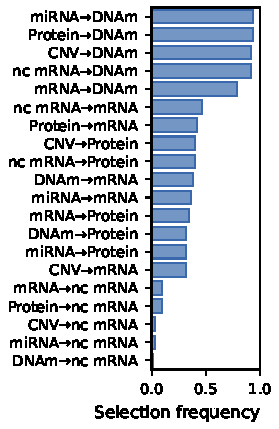
\includegraphics[scale=1]{selection_stability.pdf}
         \caption{Selection frequency of the different interactions.}
         \label{fig:alphas_stability}
     \end{wrapfigure}
     The gating block helps increase the prediction's accuracy and interpretability by highlighting the important interactions between modalities.
     In a multimodal setting, where many modalities are available, one could hypothesize that the selected interactions are random, as different modalities could provide the same amount of information.
     We trained the model fifty times to test this hypothesis and looked at the top selected interactions and their selection frequency~(\cref{fig:alphas_stability}).

     A core of 5 interactions was selected in most of the runs: Protein $\rightarrow$ DNAm, miRNA $\rightarrow$ DNAm, CNV $\rightarrow$ DNAm, nc mRNA $\rightarrow$ DNAm, mRNA $\rightarrow$ DNAm.
     These interactions are the most important as they are likely to contribute to the exploitation of complementary information between modalities.
     Some interactions were only selected in a few training runs and not considered informative for the predictions.
     Another set of interactions has a selection frequency of around 0.5.
     Those interactions probably are exploited by the model to exploit the redundancy between modalities, but they are selected randomly across the different runs.
     This suggests that they can be replaced by other interactions providing the same information level.


 \subsection{Impact of the sparsity rate}

     The \(\tau\) parameters controls the sparsity levels of the \(\alpha^{ij}\).
     Testing various sparsity rates did not impact the accuracy but did affect the number of selected interactions.
     When increasing \(\tau\), more interactions are selected.
     This observation suggests that the model is able to accommodate more interactions, but adding more interactions does not give more information as the accuracy remains similar.

     \begin{figure}[htbp]
         \begin{subfigure}[c]{0.62\textwidth}
             \centering
             \caption{}
             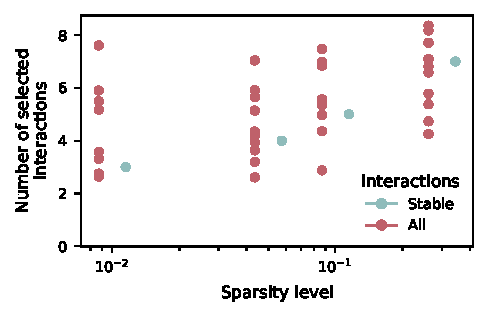
\includegraphics[width=\linewidth]{sparsity_stability.pdf}
             \label{fig:sparsity_stability}
         \end{subfigure}
         \hfill
         \begin{subtable}[c]{0.33\textwidth}
            \sisetup{separate-uncertainty-units=single, separate-uncertainty,detect-mode}
         \centering
         \label{tab:acc_sparsity}
         \begin{tblr}{
            colspec={
                Q[si={table-format=1.3,table-number-alignment=center, table-align-uncertainty = true},c, wd=1.5cm]
                Q[si={table-format=1.3(3),table-number-alignment=center, table-align-uncertainty = true}]
                },%
            row{1} = {guard, c, m},%
            row{2-Z} = {font=\small},%
            hline{1,Z} = {2pt},%
			hline{2} = {1pt},%
            }
            Sparsity rate & Accuracy          \\
            0.010         & 0.982(3) \\
            0.050         & 0.983(2) \\
            0.100         & 0.983(3) \\
            0.300         & 0.982(2) 
         \end{tblr}
         \end{subtable}
         \caption{Impact of the sparsity rate \(\tau\) on (a) the number of selected interactions and (b) the accuracy.}
     \end{figure}


 \subsection{Ablation study}
     Our training loss includes four different regularization terms.
     We performed a comprehensive ablation study to study the influence of individual regularizations.
     Three of the regularizations did not impact the accuracy but impacted the \(\alpha^{ij}\) selected~(\cref{tab:ablation_wv,tab:ablation_we,tab:ablation_wb}).
     \begin{table}[htbp]
        \centering
        \sisetup{separate-uncertainty-units=single, separate-uncertainty,detect-mode}
         \caption{Results of the ablation study of the four regularization terms.}
         \hspace{0.2\textwidth}
         \begin{subtable}[h]{0.27\textwidth}
             \caption{\(\symcal{L}_v\) ablation}\label{tab:ablation_wv}
             \begin{tblr}{
                colspec={
                    Q[si={table-format=2.1,table-number-alignment=center, table-align-uncertainty = true},c]
                    Q[si={table-format=1.3(3),table-number-alignment=center, table-align-uncertainty = true}]
                    },%
                row{1} = {guard, c, m},%
                row{2-Z} = {font=\small},%
                hline{1,Z} = {2pt},%
                hline{2} = {1pt},%
                }
                \(w_v\) & Accuracy  \\
                 0.0     & 0.982(1) \\
                 5.0     & 0.983(1) \\
                 10.0    & 0.981(1) 
             \end{tblr}
         \end{subtable}
         \hfill
         \begin{subtable}[h]{0.27\textwidth}
             \caption{\(\symcal{L}_e\) ablation}\label{tab:ablation_we}
             \begin{tblr}{
                colspec={
                    Q[si={table-format=1.2,table-number-alignment=center, table-align-uncertainty = true},c]
                    Q[si={table-format=1.3(3),table-number-alignment=center, table-align-uncertainty = true}]
                    },%
                row{1} = {guard, c, m},%
                row{2-Z} = {font=\small},%
                hline{1,Z} = {2pt},%
                hline{2} = {1pt},%
                }
                \(w_e\) & Accuracy            \\
                0.0     & 0.983(1) \\
                0.02    & 0.983(1) \\
                0.05    & 0.981(2) 
             \end{tblr}
         \end{subtable}\hspace{0.2\textwidth}

         \bigskip

         \hspace{0.2\textwidth}
         \begin{subtable}[h]{0.27\textwidth}
             \caption{\(\symcal{L}_b\) ablation}\label{tab:ablation_wb}
             \begin{tblr}{
                colspec={
                    Q[si={table-format=1.2,table-number-alignment=center, table-align-uncertainty = true},c]
                    Q[si={table-format=1.3(3),table-number-alignment=center, table-align-uncertainty = true}]
                    },%
                row{1} = {guard, c, m},%
                row{2-Z} = {font=\small},%
                hline{1,Z} = {2pt},%
                hline{2} = {1pt},%
                }
               \(w_{b}\) & Accuracy            \\
                 0.0       & 0.983(2) \\
                 0.06      & 0.983(1) \\
                 0.10      & 0.981(2) 
             \end{tblr}
         \end{subtable}
         \hfill
         \begin{subtable}[h]{0.27\textwidth}
             \caption{\(\symcal{L}_{01}\) ablation}\label{tab:ablation_w01}
             \begin{tblr}{
                colspec={
                    Q[si={table-format=1.2,table-number-alignment=center, table-align-uncertainty = true},c]
                    Q[si={table-format=1.3(3),table-number-alignment=center, table-align-uncertainty = true}]
                    },%
                row{1} = {guard, c, m},%
                row{2-Z} = {font=\small},%
                hline{1,Z} = {2pt},%
                hline{2} = {1pt},%
                }
               \(w_{01}\) & Accuracy            \\
                 0.0        & 0.977(2) \\
                 0.5        & 0.977(3) \\
                 1.0        & 0.983(1)
             \end{tblr}
         \end{subtable}\hspace{0.2\textwidth}
         \label{tab:ablation}
     \end{table}

     Firstly, we consider the impact of the \(\symcal{L}_b\) regularization by testing different values of \(w_b\).
     We find that a high value of \(w_b\) favors an important sparsity where all the alphas are close to zeros, in the range \(\left[10^{-5}; 10^{-1}\right]\).
     The absence of this regularization term limits the diversity of interactions among samples (\cref{fig:alphas_signature_ablation}).
     A larger set of \(\alpha^{ij}\) is commonly selected for different samples in this configuration.

     Secondly, we looked at the impact of \(\symcal{L}_e\) regularization by testing different values of \(w_e\).
     Similarly to \(\symcal{L}_b\), high \(w_e\) values favor more sparse solution.
     The absence of this regularization term increases the number of interactions that are selected; this term is crucial to ensure enough sparsity of the selected interactions (\cref{fig:alphas_signature_ablation}).

     \begin{figure}
         \centering
         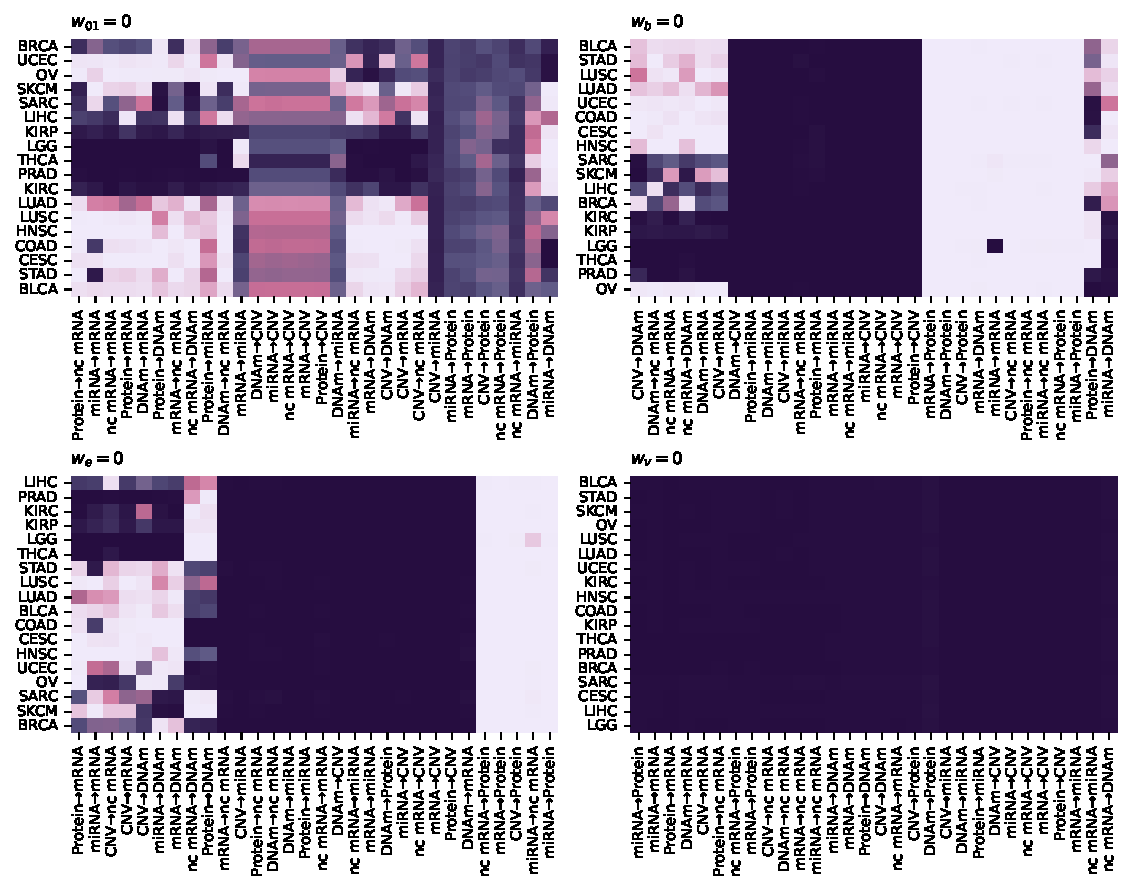
\includegraphics[width=0.7\textwidth]{ablation_heatmaps.pdf}
         \caption{Impact of the different regularization terms on the \(\alpha^{ij}\). (Top left) Impact of the \(\symcal{L}_{01}\) regularization. (Top right) Impact of the \(\symcal{L}_{b}\) regularization. (Bottom left) Impact of the \(\symcal{L}_{e}\) regularization. (Bottom right) Impact of the \(\symcal{L}_{v}\) regularization.}
         \label{fig:alphas_signature_ablation}
     \end{figure}

     The \(\symcal{L}_v\) is essential to counterbalance the sparsity and ensure there is enough diversity among the selected \(\alpha^{ij}\).
     In the absence of the \(\symcal{L}_v\), \(w_v = 0\), only the regularization terms controlling the sparsity are applied.
     The solution that is obtained is a solution with a maximum of \(\alpha^{ij}\)  as close as possible to zero to fulfill the sparsity constraints (\cref{fig:alphas_signature_ablation}).
     \(\alpha^{ij}\) that are not set to zeros have small values in the range \(\left[10^{-5}; 10^{-2}\right]\).
     On the contrary, high values of \(w_v\) favor more diversity among the selected \(\alpha^{ij}\) but with a lower sparsity.
     To ensure the diversity constraints, more \(\alpha^{ij}\) are selected.

     The absence \(\symcal{L}_{01}\) regularization reduced the accuracy and reduced the sparsity of the selected \(\alpha^{ij}\) (\cref{tab:ablation_w01,fig:alphas_signature_ablation}).
     This regularization term is essential in the correct training of the gating mechanism.

     It is necessary to balance those regularization terms to ensure enough diversity and sparsity.

 \subsection{Comparison with post-hoc methods}

     We compare our approach with post-hoc methods.
     A model with no gate is trained, and we used LRP to estimate the importance score of each interaction (\cref{fig:signature_LRP}).

     \begin{figure}[htbp]
         \centering
         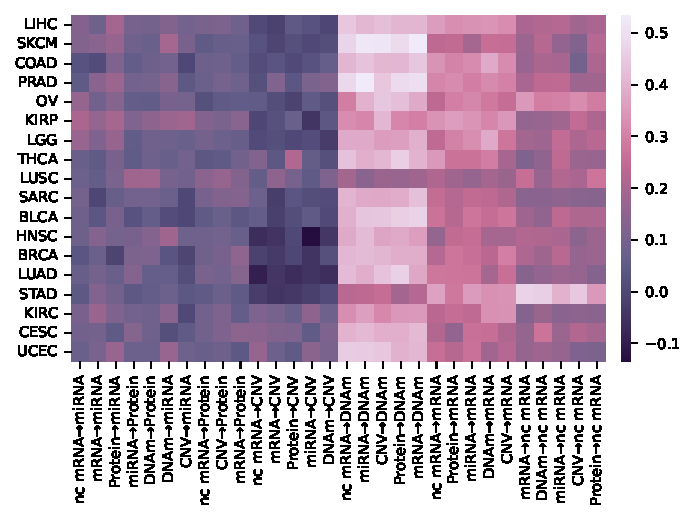
\includegraphics[scale=0.75]{signature_alphas_LRP.pdf}
         \caption{LRP importance score for the different modalities interactions.}\label{fig:signature_LRP}
     \end{figure}

     With LRP, all interactions contribute to the predictions to some extent.
     This approach is less interpretable as no clear signature can be distinguished for each cancer.
     In the absence of the gating mechanism, all interactions are used to perform predictions; there is no sparsity.
     The LRP importance score for each interaction is similar across phenotypes; there is no diversity.
     The importance score variance across samples was around 0.1, whereas, with our approach, the diversity was higher, with variances up to 0.5.

\section{Conclusion}
 This chapter introduced a new interpretable multimodal architecture.
 The model is interpretable by construction thanks to a gating mechanism that scores the interactions of different modalities.
 We showed that the gating mechanism improves both accuracy and interpretability compared to our baseline.
 Gate importance scores must be sparse to ensure correct interpretability and diversity to reflect the diversity that exists between samples.
 To ensure these two properties are met, we added four regularization terms to our training process.
 Our ablation study showed that the four terms are essential to ensure both sparsity and diversity while improving accuracy.
 While we tested our architecture in the healthcare domain on omics datasets, the architecture presented in this paper can be applied to any domain with high-dimensional multimodal data.
\end{document}
